\section{Análisis de precisión de heurísticas}

Dado que el objetivo de este TP es encontrar la mejor solución posible sin utilizar algoritmos exactos (ya que el problema en sí se resuelve en tiempo exponencial), nos dispusimos a comprar los resultados obtenidos entre todos los algoritmos, poniendo énfasis en la precisión de los resultados y su relación con el tiempo de ejecución de cada uno. La idea es hallar el algoritmo que mantenga la mejor proporción tiempo-calidad.

De cara a esto, sabemos que la heurística golosa es la más veloz. También suponemos que la aplicación de la metaheurística GRASP puede incrementar ampliamente la calidad de la solución (si se seleccionan correctamente los parámetros que la misma utiliza).

Para estos tests, se generaron nuevamente grafos en base a distribuciones uniformes tales que:

\begin{itemize}
	\item $n \leq 40$
	\item $m \leq \frac{n * (n-1)}{4}$
\end{itemize}

Esto se debe a que los resultados deben ser comparados con los del algoritmo exacto, lo cual restringe el tamaño de los grafos a generar (o su solución no podría hallarse en tiempo razonable).

Además de hacer pruebas generales, se hicieron algunas pruebas específicas a los casos patológicos. Estos fueron generados con las siguientes propiedades (detalles adicionales sobre el funcionamiento de estos generadores se encuentran en el apéndice):

\begin{itemize}
    \item $k \leq 15$
    \item $q == 10$ (exclusivamente para GRASP)
\end{itemize}

Para cada heurística, analizaremos los siguientes aspectos de las pruebas:

\begin{itemize}
	\item el porcentaje de resultados que difieren con la solución exacta (independientemente de la diferencia real),
	\item el error máximo realizado por el algoritmo,
	\item el error promedio de todos los casos (esto incluye aqueyos sin error),
	\item la desviación estandar de dicha diferencia, y
    \item el tiempo de ejecución promedio de las heurísticas
\end{itemize}

Creemos que con estos indicadores, podemos analizar correctamente el comportamiento de cada algoritmo y realizar comparaciones entre los mismos.

\subsection*{Heurística constructiva golosa}

Primero decidimos mirar la heurística golosa, ya que las otras están pensadas para funcionar sobre la misma:

\begin{center}
    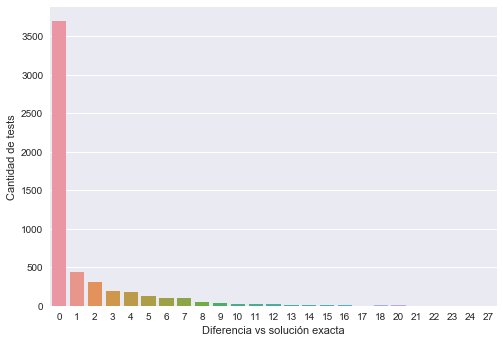
\includegraphics[scale=0.6]{img/accuracy-greedy.png}
\end{center}

A simple vista, en promedio, la heurística parece bastante precisa. De base podemos ver que el enfoque es efectivo para resolver el algoritmo, aunque no necesariamente suficiente. De estas pruebas pudimos extraer los siguientes indicadores:

\begin{center}
    \begin{tabular}{ | l l |}
        \hline
        Porcentaje de resultados con error & 30.83\% \\ \hline
        Errores & $\Delta$ \\
        - máximo & $max(\Delta) = 24$ \\
        - promedio & $\mu(\Delta) = 1.18$ \\
        - desviacion estandar & $\sigma(\Delta) = 2.52$ \\ \hline
        Tiempo (en ns) & $\Delta$ \\
        - máximo & $max(t) = 31079 $ \\
        - promedio & $\mu(t) = 10122.04$ \\
        - desviacion estandar & $\sigma(t) = 6429.43$ \\
        \hline
    \end{tabular}
\end{center}

Como podemos ver, la heurística golosa de por sí no es tan exacta, aunque en promedio los errores son menores. Si miramos especificamente los casos patológicos del enfoque goloso:

\noindent
\begin{minipage}{0.55\textwidth}
    \hfill
    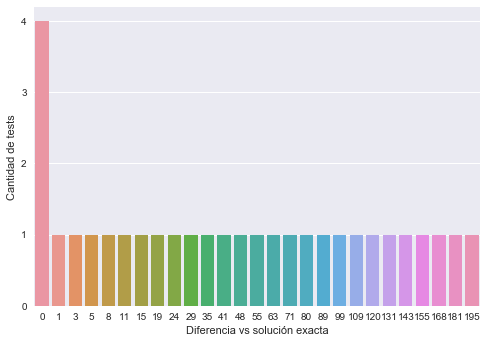
\includegraphics[scale=0.6]{img/path-greedy.png}
\end{minipage}
\hfill
\begin{minipage}{0.44\textwidth}
    \begin{center}

        \begin{tabular}{ | l l |}
            \hline
            \% de resultados & \\
            con error & 86.67\% \\ \hline
            Errores & $\Delta$ \\
            - máximo & $max(\Delta) = 195$ \\
            - promedio & $\mu(\Delta) = 63.27$ \\
            - desviacion estandar & $\sigma(\Delta) = 61.71$ \\ \hline
            Tiempo (en ns) & t \\
            - máximo & $max(t) = 13200 $ \\
            - promedio & $\mu(t) = 7102.53$ \\
            - desviacion estandar & $\sigma(t) = 3629.22$ \\
            \hline
        \end{tabular}
    \end{center}
\end{minipage}

Podemos ver que en estos casos, el algoritmo comete errores enormes, y en general no encuentra el caso ideal. Para grafos de menor tamaño, el caso patológico no es tal, pero a medida que aumenta el tamaño del grafo, la solución es relativamente peor.

Cabe destacar que al analizar los tiempos de ejecución, el caso patológico no es necesariamente más lento que un grafo promedio de tamaño equivalente. Si bien los tiempos de ejecución no son comparables por los distintos tamaños, en general la calidad del resultado no influye (al menos de forma negativa) en los tiempos de ejecución. 

\subsection*{Heurística de búsqueda local}

\begin{center}
    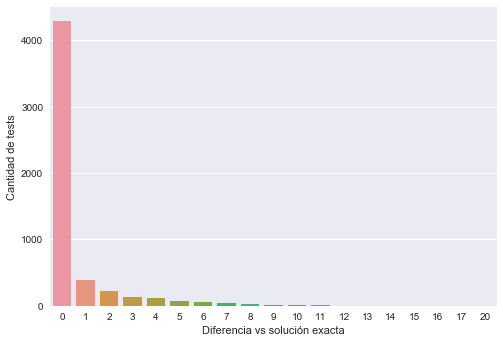
\includegraphics[scale=0.6]{img/accuracy-local.png}
\end{center}

Al aplicar una búsqueda local sobre la metodología greedy, podemos ver una amplia mejoría de los resultados obtenidos. La misma se evidencia mejor en los indicadores:

\begin{center}
    \begin{tabular}{ | l l |}
        \hline
        Porcentaje de resultados con error & 20.21\% \\ \hline
        Errores & $\Delta$ \\
        - máximo & $max(\Delta) = 15$ \\
        - promedio & $\mu(\Delta) = 0.59$ \\
        - desviacion estandar & $\sigma(\Delta) = 1.56$ \\ \hline
        Tiempo (en ns) & $\Delta$ \\
        - máximo & $max(t) = 1886955 $ \\
        - promedio & $\mu(t) = 189041.69$ \\
        - desviacion estandar & $\sigma(t) = 202448.43$ \\
        \hline
    \end{tabular}
\end{center}

En promedio, el error cae por debajo de 1, y la cantidad de casos con resultado exacto aumenta significativamente. Sin embargo, sigue habiendo varios errores, incluyendo algunas diferencias grandes.

\noindent
\begin{minipage}{0.55\textwidth}
    \hfill
    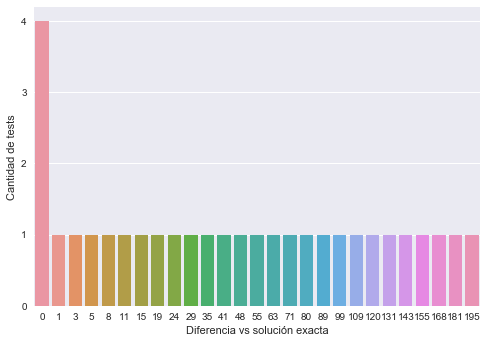
\includegraphics[scale=0.6]{img/path-local.png}
\end{minipage}
\hfill
\begin{minipage}{0.44\textwidth}
    \begin{center}

        \begin{tabular}{ | l l |}
            \hline
            \% de resultados & \\
            con error & 86.67\% \\ \hline
            Errores & $\Delta$ \\
            - máximo & $max(\Delta) = 195$ \\
            - promedio & $\mu(\Delta) = 63.27$ \\
            - desviacion estandar & $\sigma(\Delta) = 61.71$ \\ \hline
            Tiempo (en ns) & t \\
            - máximo & $max(t) = 46304 $ \\
            - promedio & $\mu(t) = 25391.73$ \\
            - desviacion estandar & $\sigma(t) = 12556.97$ \\
            \hline
        \end{tabular}
    \end{center}
\end{minipage}

Desafortunadamente, en el caso del grafo patológico, los resultados son exactamente iguales, ya que la forma del grafo no permite intercambiar un único nodo e incrementar la frontera, resultando en un máximo local que no puede mejorar.

No solo eso, dado que el grado máximo es muy elevado, el tiempo de ejecución se triplica en promedio al de la heurística golosa, ya que busca mejoría entre sus nodos adyacentes y se haya con muchos casos idénticamente malos.

\subsection*{Metaheurística GRASP}

Al analizar la precisión de GRASP, tuvimos que tener en cuenta los parámetros de la metaheurística: el porcentaje de los nodos considerados y la cantidad de iteraciones aleatorias. La combinatoria de estos dos parámetros es muy grande, así que decidimos mostrar solo algunos de los valores que consideramos representativos de las tendencias generales:

\begin{center}
    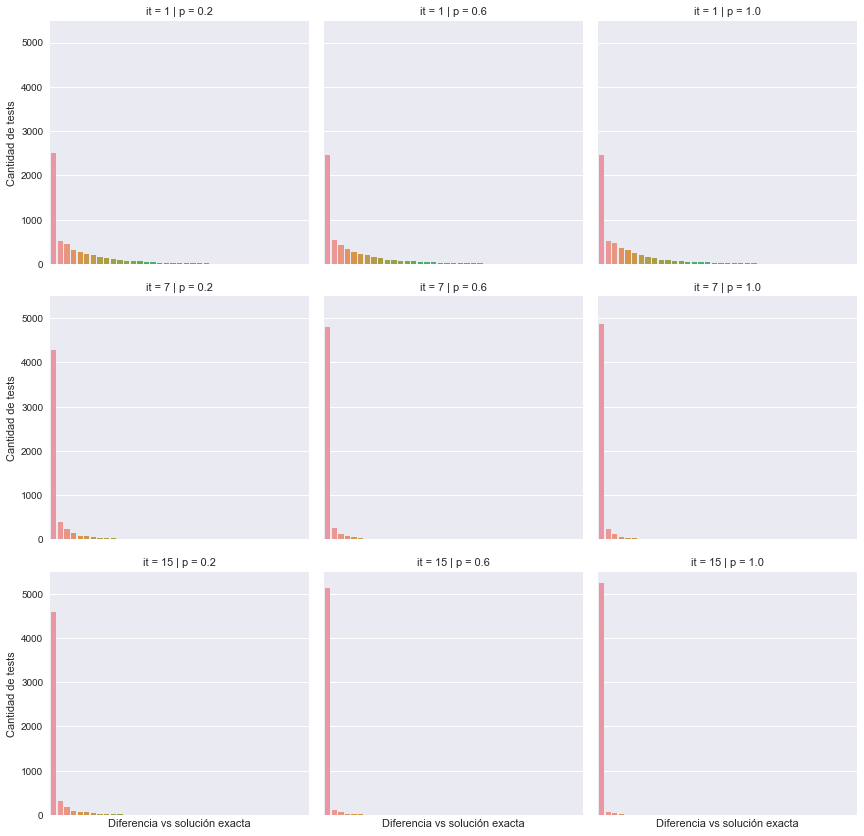
\includegraphics[scale=0.6]{img/accuracy-grasp-3x3.png}
\end{center}

Si bien este gráfico no permite un análisis muy profundo, muestra una tendencia básica: mientras más iteraciones se realizan, más errores se depuran, y la solución se aproxima más al resultado exacto. No solo eso, realizando una única iteración, los resultados de la metaheurística son paupérrimos. Esto se debe a que la instancia golosa tomada es aleatoria, por lo que varía con respecto a su contraparte estrictamente golosa, y suele ser peor aunque puede superar.

\begin{center}
    \begin{tabular}{ | c | c | c | c | c | c | c |}
        \hline
        \% de nodos considerados & Iteraciones & \% de error & $max(\Delta)$ & $\mu(\Delta)$ & $\sigma(\Delta)$ & $\mu(t)$ \\ \hline
            &  1 & 68.3\% & 48 & 4.556 & 5.658 &  318434 \\ \cline{2-7}
        0.2 &  7 & 21.0\% & 27 & 0.696 & 1.939 & 2351098 \\ \cline{2-7}
            & 15 & 17.5\% & 18 & 0.530 & 1.598 & 5021068 \\ \hline
            &  1 & 75.9\% & 59 & 5.861 & 6.489 &  281990 \\ \cline{2-7}
        0.6 &  7 & 11.8\% & 15 & 0.307 & 1.133 & 2339655 \\ \cline{2-7}
            & 15 &  4.7\% &  9 & 0.097 & 0.562 & 5009071 \\ \hline
            &  1 & 78.9\% & 60 & 6.484 & 6.789 &  260273 \\ \cline{2-7}
          1 &  7 &  9.3\% & 13 & 0.227 & 0.952 & 2350323 \\ \cline{2-7}
            & 15 &    2\% &  9 & 0.054 & 0.401 & 4995022 \\
        \hline
    \end{tabular}
\end{center}

Mirando un poco más de cerca los datos obtenidos, se ve de manera mucho más clara en qué influye cada parámetro. En particular, podemos destacar algunas cosas:

\begin{enumerate}
    \item el factor aleatorio de GRASP puede derivar en resultados menos fiables que usando una heurística golosa simple o con búsqueda local;
    \item por este factor aleatorio de GRASP puede derivar en resultados menos fiables que usando una heurística golosa simple o con búsqueda local;
	\item si bien el porcentaje de nodos considerados influye en la tasa de error, la cantidad de iteraciones realizadas tiene un impacto mucho más visible, y es lo que permite a GRASP obtener mejores resultados que greedy, utilizando el aspecto random de manera ventajosa en lugar de generar casos patológicos;
    \item más allá de lo recíén dicho, la cantidad de iteraciones sigue una suerte de ley de retornos decrecientes, y aumentar la cantidad de repeticiones linealmente no genera resultados linealmente mejores, ya que las instancias aleatorias comienzan a repetirse; y
    \item por este factor aleatorio, el tiempo de ejecución disminuye al aumentar p ya que se consideran casos subóptimos con cliques más pequeñas, que resultan en menor tiempo de ejecución de la contrucción golosa.
\end{enumerate}

Entre estos casos particulares, los parámetros que mejores resultados brindan son $p = 1$ e $it = 15$. Muy cerca de estos resultados se encuentra $p = 0.6$ e $it = 15$, que en promedio dan peores resultados con un costo de ejecución comparable o peor.

A modo de comparación con las pruebas realizadas en la sección de la metaheurística, probamos los parámetros particulares que fueron entregados con el ejecutable de este TP: $p = 0.6$ e $it = 50$.

\noindent
\begin{minipage}{0.55\textwidth}
    \hfill
    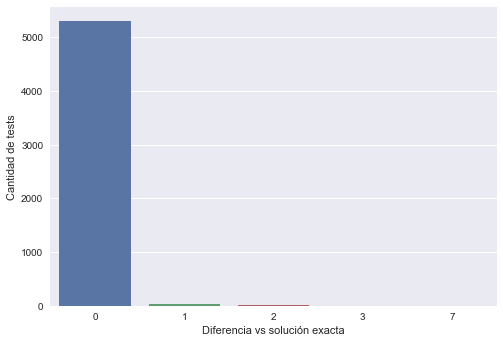
\includegraphics[scale=0.55]{img/accuracy-grasp50.png}
\end{minipage}
\hfill
\begin{minipage}{0.44\textwidth}
    \begin{center}

        \begin{tabular}{ | l l |}
            \hline
            \% de resultados con error & 1.04\% \\ \hline
            Errores & $\Delta$ \\
            - máximo & $max(\Delta) = 6$ \\
            - promedio & $\mu(\Delta) = 0.018$ \\
            - desviacion estandar & $\sigma(\Delta) = 0.21$ \\
            \hline
        \end{tabular}
    \end{center}
\end{minipage}

Como se puede notar, el resultado es mucho más preciso que algunos de los casos mostrados anteriormente. Es más, en este caso, aumentar las iteraciones de 15 a 50 (resultando en más del triple del tiempo de ejecución) produjo una diferencia de calidad porcentualmente visible (se redujeron los errores a la mitad, con mucho menor promedio y desviación).

Sin embargo, en términos netos, la diferencia no es tanta, ya que con muchas menos iteraciones la heurística estaba generando buenos resultados. Es difícil cuantificar esta diferencia, ya que depende mucho de los casos de prueba provistos y de la precisión deseada, pero vale la pena mencionar que este aumento en tiempo de ejecución podría no ser valioso.

En cuanto a los casos patológicos, primero decidimos comparar el rendimiento de GRASP frente al caso base que afecta a las heurísticas golosa y de búsqueda local:

\begin{center}
    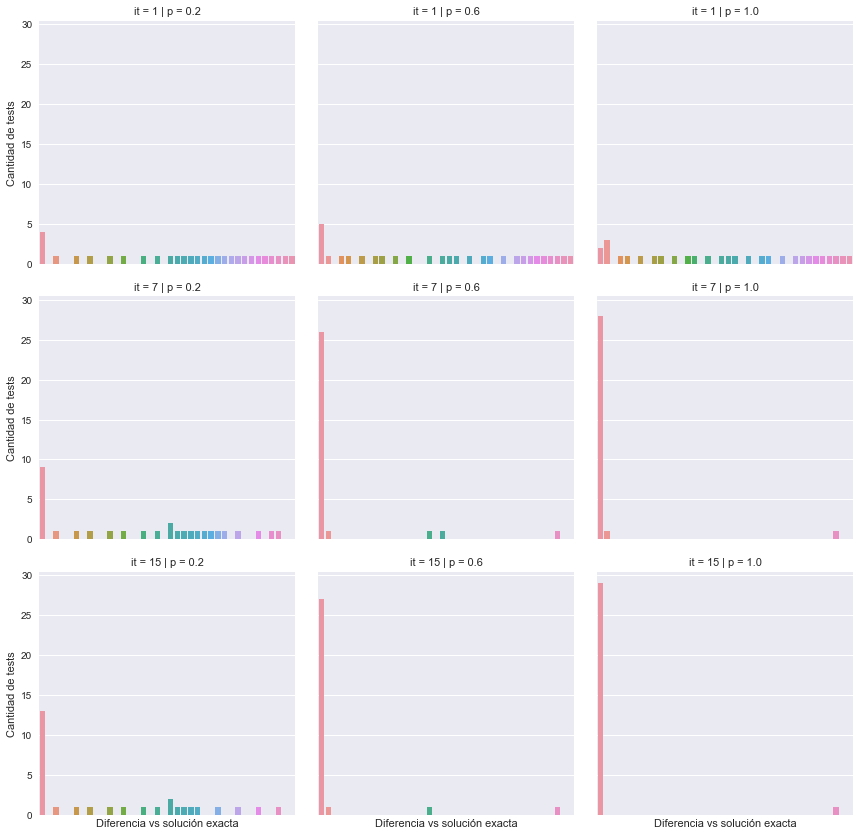
\includegraphics[scale=0.6]{img/path-grasp-3x3.png}

    \begin{tabular}{ | c | c | c | c | c | c | c |}
        \hline
        \% de nodos considerados & Iteraciones & \% de error & $max(\Delta)$ & $\mu(\Delta)$ & $\sigma(\Delta)$ & $\mu(t)$ \\ \hline
            & 1  & 59.1\% & 195 & 43.136 & 58.795 & 1185127  \\ \cline{2-7}
        0.2 & 7  & 52.5\% & 168 & 28.750 & 45.273 & 5662686  \\ \cline{2-7}
            & 15 & 47.2\% & 168 & 20.972 & 39.199 & 14800435 \\ \hline
            & 1  & 45.5\% & 195 & 33.982 & 55.472 & 1184289  \\ \cline{2-7}
        0.6 & 7  & 11.8\% & 168 & 7.206  & 29.831 & 7958280  \\ \cline{2-7}
            & 15 &  9.1\% & 168 & 6.182  & 29.680 & 19987087 \\ \hline
            & 1  & 48.3\% & 195 & 32.759 & 54.334 & 1187642  \\ \cline{2-7}
        1   & 7  &  6.2\% & 168 & 5.281  & 29.693 & 10044562 \\ \cline{2-7}
            & 15 &  3.2\% & 168 & 5.419  & 30.174 & 22387163 \\
        \hline
    \end{tabular}
\end{center}

Estos resultados fueron muy interesantes porque, a diferencia de la tendencia vista en promedio, el tiempo de ejecución aumentó junto con $p$. Esto se debe a la distribución de los ejes en nuestro grafo: ya que el nodo de mayor grado solo permite generar cliques pequeñas, y cada nodo debe ser comparado contra aquellos que forman la solución, los ciclos del algoritmo goloso son más cortos.

Al probar con los parámetros entregados en el ejecutable del TP ($p = 0.6, it = 50$), logramos eliminar todos los errores, pero debemos recalcar que el tiempo de ejecución es más del triple, lo cual puede ser prohibitivo dependiendo del contexto.

Por último, decidimos generar casos patológicos especificamente diseñados para GRASP. La lógica interna es similar a la de los casos patológicos de las otras heurísticas, pero con el adicional de agregar múltiples falsos positivos (componentes estrella) en un intento de aumentar la probabilidad de que sean seleccionados, generando malos resultados.


\begin{center}
    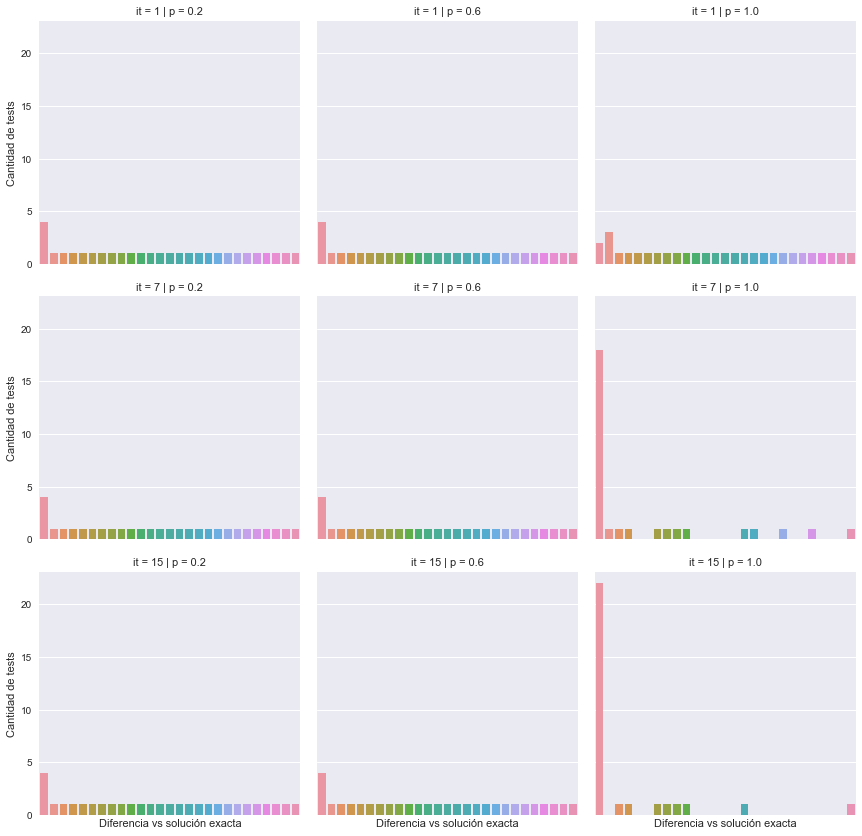
\includegraphics[scale=0.6]{img/path-grasp2-3x3.png}
    
    \begin{tabular}{ | c | c | c | c | c | c | c |}
        \hline
        \% de nodos considerados & Iteraciones & \% de error & $max(\Delta)$ & $\mu(\Delta)$ & $\sigma(\Delta)$ & $\mu(t)$ \\ \hline
            & 1  & 86.7\% & 195 & 63.267 & 61.710 &   66185 \\ \cline{2-7}
        0.2 & 7  & 86.7\% & 195 & 63.267 & 61.710 &  975937 \\ \cline{2-7}
            & 15 & 86.7\% & 195 & 63.267 & 61.710 & 2254688 \\ \hline
            & 1  & 76.5\% & 195 & 55.824 & 61.438 &  185755 \\ \cline{2-7}
        0.6 & 7  & 74.3\% & 195 & 54.229 & 61.259 & 1430836 \\ \cline{2-7}
            & 15 & 74.3\% & 195 & 54.229 & 61.259 & 3068547 \\ \hline
            & 1  & 49.1\% & 195 & 33.333 & 54.639 &  285059 \\ \cline{2-7}
        1   & 7  & 28.6\% & 195 & 16.524 & 42.012 & 1683083 \\ \cline{2-7}
            & 15 & 21.6\% & 195 &  9.757 & 33.986 & 4033435 \\
        \hline
    \end{tabular}
\end{center}

Aquí es claro el rol del parámetro $p$ en la heurística. Si bien existen casos (en particular, casos favorables para la heurística golosa) donde considerar más nodos resulta en una pérdida de tiempo y resultados menos fiables, en estos casos se ve exactamente lo opuesto: considerar la mayor cantidad de nodos resulta en resultados más precisos, ya que la cantidad de falsos positivos es muy grande.

Por supuesto, debe recordarse que GRASP tiene un alto componente aleatorio: así como $p = 1, it = 1$ superó otras instancias con menor $p$ y más iteraciones, podría haber resultado en valores igualmente malos.

\subsection*{Resumen comparativo y conclusiones}

A modo de referencia, se muestra aquí una comparación entre todas las heurísticas analisadas:

\bigskip

\begin{tabular}{| l | r | r | r | r | r | r | r | r |}
    \hline
                             & \multicolumn{4}{|c|}{Gráfos uniformes}                            & \multicolumn{4}{|c|}{Gráfos patológicos}    \\ \cline{2-9}
    Heurística               & \% error & $\mu(\Delta)$ & $\sigma(\Delta)$ & $\mu(t)$ & \% error & $\mu(\Delta)$ & $\sigma(\Delta)$ & $\mu(t)$ \\ \hline
    Constructiva Golosa      &  30.83\% &          1.18 &             2.52 &    10122 &  86.67\% &         63.27 &            61.71 &     7102 \\ \hline
    Búsqueda Local           &  20.21\% &          0.59 &             1.56 &   189041 &  86.67\% &         63.27 &            61.71 &    25391 \\ \hline
    GRASP (p = 1, it = 15)   &      2\% &          0.05 &             0.40 &  4995022 &   21.6\% &          9.76 &            33.99 &  4033435 \\ \hline
    GRASP (p = 0.6, it = 50) &   1.04\% &          0.02 &             0.21 & 99235601 &     70\% &         35.20 &            41.47 &  6918257 \\
    \hline
\end{tabular}

Como se puede ver, el uso de heurísticas más complejas conlleva un gran aumento del tiempo de ejecución. Algo que nos llamó la atención fue hecho que la búsqueda local, si bien mejora los resultados, tiene un gran costo relativo a los errores resueltos, y sufre los mismos casos patológicos. Por otro lado, la metaheurística reduce ampliamente los errores, pero su uso de búsquedas locales y el factor aleatorio significan que debe ser usado con precaución.

Otro detalle interesante es como el tiempo de ejecución de GRASP puede resultar inversamente proporcional a la calidad del resultado hallado: si bien realizamos más del triple de iteraciones, al utlizar un p menor y no hallar el caso óptimo cada iteración tarda menos porque las cliques a considerar son más pequeñas.

En conclusión, el uso de una metaheurística puede brindar resultados muy cercanos a un algoritmo preciso, pero debe ser optimizada con cuidado en cada uno de sus componentes (incluyendo tanto sus parámetros como sus heurísticas internas) para que el costo de ejecución a pagar por soluciones de mayor calidad no sea muy alto. 